\documentclass{article}
\usepackage[utf8]{inputenc}
\usepackage{amsmath,amsfonts,amsthm,amssymb,xcolor,tikz}
% math font macros

% bb
\newcommand{\NN}{\mathbb{N}}
\newcommand{\ZZ}{\mathbb{Z}}
\newcommand{\QQ}{\mathbb{Q}}
\newcommand{\RR}{\mathbb{R}}
\newcommand{\CC}{\mathbb{C}}
\newcommand{\PP}{\mathbb{P}}
\newcommand{\PC}{\PP \,(\CC)}
\newcommand{\AAA}{\mathbb{A}}
\newcommand{\EE}{\mathbb{E}}

% calligraphic
\newcommand{\calF}{{\mathcal F}}
\newcommand{\calA}{\mathcal{A}}
\newcommand{\calB}{\mathcal{B}}
\newcommand{\calO}{\mathcal{O}}
\newcommand{\variety}{\mathcal{V}}
\newcommand{\ideal}{\mathcal{I}}
\newcommand{\bs}{\boldsymbol}

% fraktur
\newcommand{\frakv}{\mathfrak{v}}
\newcommand{\frakm}{\mathfrak{m}}

% text color
\newcommand{\red}{\textcolor{red}}
\newcommand{\orange}{\textcolor{orange}}
\newcommand{\blue}{\textcolor{blue}}

% math operators
\DeclareMathOperator{\len}{\rm len}
\DeclareMathOperator{\trop}{\rm trop}
\DeclareMathOperator{\Gr}{Gr}
\DeclareMathOperator{\Div}{\rm Div}
\DeclareMathOperator{\Cl}{\rm Cl}
\DeclareMathOperator{\divisor}{\rm div}
\DeclareMathOperator{\Var}{\rm Var}
\DeclareMathOperator{\Exp}{\rm Exp}
\DeclareMathOperator{\ev}{\rm ev}
\DeclareMathOperator{\supp}{\rm supp}
\DeclareMathOperator{\Vol}{\rm Vol}
\DeclareMathOperator{\ind}{\rm ind}
\DeclareMathOperator{\im}{\rm im}
\DeclareMathOperator{\Cone}{\rm Cone}
\DeclareMathOperator{\spec}{\rm Spec}
\DeclareMathOperator{\spa}{\rm span}
\DeclareMathOperator{\conv}{\rm conv}
\DeclareMathOperator{\err}{\rm err}
\DeclareMathOperator{\gr}{\rm gr}
\DeclareMathOperator{\rk}{{\rm rank}}

% theorem declarations
\newtheorem{thm}{Theorem}
\newtheorem{prop}{Proposition}
\theoremstyle{definition}
\newtheorem{example}{Example}
\newtheorem{defn}{Definition}
\newtheorem{remark}{Remark}



\title{Macaulay2 Exercises}
\author{Tim Duff}
\date{December 2018}

\begin{document}

\maketitle
$ $\\
Instructions: Pick the problem that interests you most and try to solve it. Maybe try to work in groups. That can be fun sometimes... The problems are categorized as follows:
\begin{itemize}
    \item[1] Gr\"{o}bner basics
    \item[2] General programming
    \item[3] Intersection Theory
    \item[4] Numerical Algebraic Geometry
    \item[5] Local computations
    \item[6] Discrete / tropical
    \item[7] Hilbert functions / free resolutions
\end{itemize}
1) a) For $i=1,2,3,$ consider affine quadrics defined by
\[
f_i (x_1,x_2) = a_i \, (x_1^2+x_2^2) + b_i \, x_1  + c_i \, x_2.
\]
The locus of $\left( [a_1:b_1:c_1], [a_2:b_2:c_2], [a_3: b_3: c_3] \right)\in \PP^2 \times \PP^2 \times \PP^2$ such that the $f_i$ meet in some point other than $(0,0) \in \AAA^2$ is Zariski closed. What is its dimension? Defining equation(s)? Use Macaulay2 or geometric argument---then try the other way.\\\
b) Analagously, we may ask about when homogeneous quadrics
\[
h_i (x_0,x_1,x_2) = a_i \,  (x_1^2+x_2^2) + b_i\, x_0 x_1 + c_i\, x_0 x_2.
\]
for $i=1,2,3$ meet in some point other than $[1:0:0]\in \PP^2.$ Does anything change? How might you relate problems a) and b)?\\\\
2) We can represent a binary tree by a \texttt{MutableList}. For example, to represent the tree below, 
\begin{center}
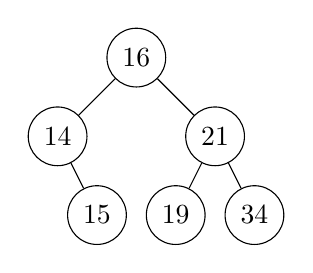
\begin{tikzpicture}
\node[circle, draw] (n1) at (0,0) {$16$};
\node[circle, draw] (n2) at (-1,-1) {$14$};
\node[circle, draw] (n3) at (1, -1) {$21$};
\node[circle, draw] (n5) at (-.5, -2) {$15$};
\node[circle, draw] (n6) at (.5, -2) {$19$};
\node[circle, draw] (n7) at (1.5, -2) {$34$};
\path (n1) edge (n2);
\path (n1) edge (n3);
\path (n2) edge (n5);
\path (n3) edge (n6);
\path (n3) edge (n7);
\end{tikzpicture}
\end{center}
we may use the following code:
\begin{verbatim}
    > M = new MutableList from {}
    > scan({0,1,2,4,5,6}, 
           {16,14,21,15,19,34},
           (i,x) -> M#i = x
           )
    \end{verbatim}
\end{verbatim}
The example above is a \emph{binary search tree}: for every node, its key is $\ge$ all keys in its left subtree and $\le $ all keys in its right subtree.\\\\
a) Write a a method function \texttt{inorder} with the following methods
\begin{itemize}
    \item \textt{inorder (MutableList, ZZ)} --- efficiently prints, in ascending numerical order, all keys in the subtree of a mutable list which is rooted at a particular index (assuming the MutableList represents a BST)
    \item \texttt{inorder MutableList} --- prints all keys in order
\end{itemize}
b) Assuming the BST property holds for your input, write an efficient function that searches for a node with a particular key\\\\
c) Write an efficient function that inserts an integer while maintaing the BST property\\\\
d) Wrap your code in a \texttt{new Type of MutableList}, and re-implement methods for for this new ``class" which solve a, b, and c.\\\\
3) a) Look up the documentation for the package \texttt{Schubert2}. How is the Chow Ring of a Grassmannian represented? What are the methods for \texttt{chern} and \texttt{schubertCycle}? What do the commands \texttt{bundles} and \texttt{integral} do?\\\\
b) How would we use Schubert2 calculate the number of lines on a generic quintic threefold in $\PP^4?$ (Hint: it is in the documentation.) Find a friend who chose problem 4b) and compare answers.\\\\
c) How many lines in $\PP^5$ meet 4 general 2-planes?\\\\
d) How many lines in $\PP^2$ meet 8 general 3-planes?\\\\
4) a) Use \texttt{NumericalAlgebraicGeometry} to study the polynomial system $x^2y+2xy^2+xy-1=x^2y-xy^2-xy+2=0.$ Bezout's theorem predicts a certain number of solutions. Do you count the same number? What is the source of the discrepency, if any? \\\\
b) Download the starter code for this problem on github. Try to understand what it does. How many lines are on a generic quintic threefold in $\PP^4?$ Find a friend who chose problem 3b) and compare answers.\\\\
5) Look up the Eisenbud-Levine-Khimshiashvili signature formula on wikipedia. There is a detailed description of how to compute the local degree of the map $\RR^2 \ni (x,y) \mapsto (x^3 - 3 x y^2, 3 x^2 y - y^3) \in \RR^2$ near $(0,0).$ Can you replicate this calculation using Macaulay2?\\\\
6) a) For fixed $k\ge 3,$ consider the locus of $(a,b,c)$ for which the polynomial $x^{2^k} + a x^{2^{k-1}} + b x^{2^{k-2}} + c$ has a double root. This should be a affine hypersurface---can you predict its Newton polytope?\\\\
b) For $n\ge 3,$ how many cones of maximum dimension are in the tropical variety $\trop \left( \langle x_{1, i} + x_{1,j } - x_{i, j} \mid 2 \le i < j \le n \rangle \right)? $\footnote{Problem source:  \hyperlink{https://icerm.brown.edu/programs/sp-f18/w4/files/day1/Problems-by-Diane.pdf})}\\\\
7) a) Explain what the code below does 
\begin{verbatim}
R = QQ[x_0,x_1,x_2]

pointIdeal = m -> (
    assert(numrows m == 2);
    minors(2, (m||matrix{{1}}) | transpose vars R)

pointsIdeal = m -> (
    t := rank source m;
    J := pointIdeal(m_{0});
    scan(t-1, i -> J = intersect(J, pointIdeal(m_{i+1})));
    J
    )
\end{verbatim}
b) Suppose $X$ is a set of $6$ points in $\PP^2.$ The structure of the homogeneous coordinate ring $k[x_0,x_1,x_2]/I_X$ depends on which subsets of points in $X$ are collinear. Write down all possible Hilbert functions for $X.$ Do the same for Betti tables. Which different configurations give the same invariants?\footnote{Problem source: http://citeseerx.ist.psu.edu/viewdoc/download?doi=10.1.1.57.7472&rep=rep1&type=pdf}
\end{document}
